
\documentclass[11pt,letterpaper]{article}

% Load some basic packages that are useful to have
% and that should be part of any LaTeX installation.
%
% be able to include figures
\usepackage{graphicx}
% get nice colors
\usepackage{xcolor}

% change default font to Palatino (looks nicer!)
\usepackage[latin1]{inputenc}
\usepackage{mathpazo}
\usepackage[T1]{fontenc}
% load some useful math symbols/fonts
\usepackage{latexsym,amsfonts,amsmath,amssymb}

% comfort package to easily set margins
\usepackage[top=1in, bottom=1in, left=1in, right=1in]{geometry}

% control some spacings
%
% spacing after a paragraph
\setlength{\parskip}{.15cm}
% indentation at the top of a new paragraph
\setlength{\parindent}{0.0cm}


\begin{document}

\begin{center}
\Large
Ay190 -- Worksheet 6\\
Anthony Alvarez\\
Date: January 28, 2014
\end{center}

\section{Linear Regression}
\subsection{Loading Data}

After successfully loading the data into python we are able to plot it and 
examine its proporties. In figures ~\ref{fig:data} we can see that the data 
is fairly linear and therefore will be fit by a line fairly well.

\begin{figure}[bth]
\centering
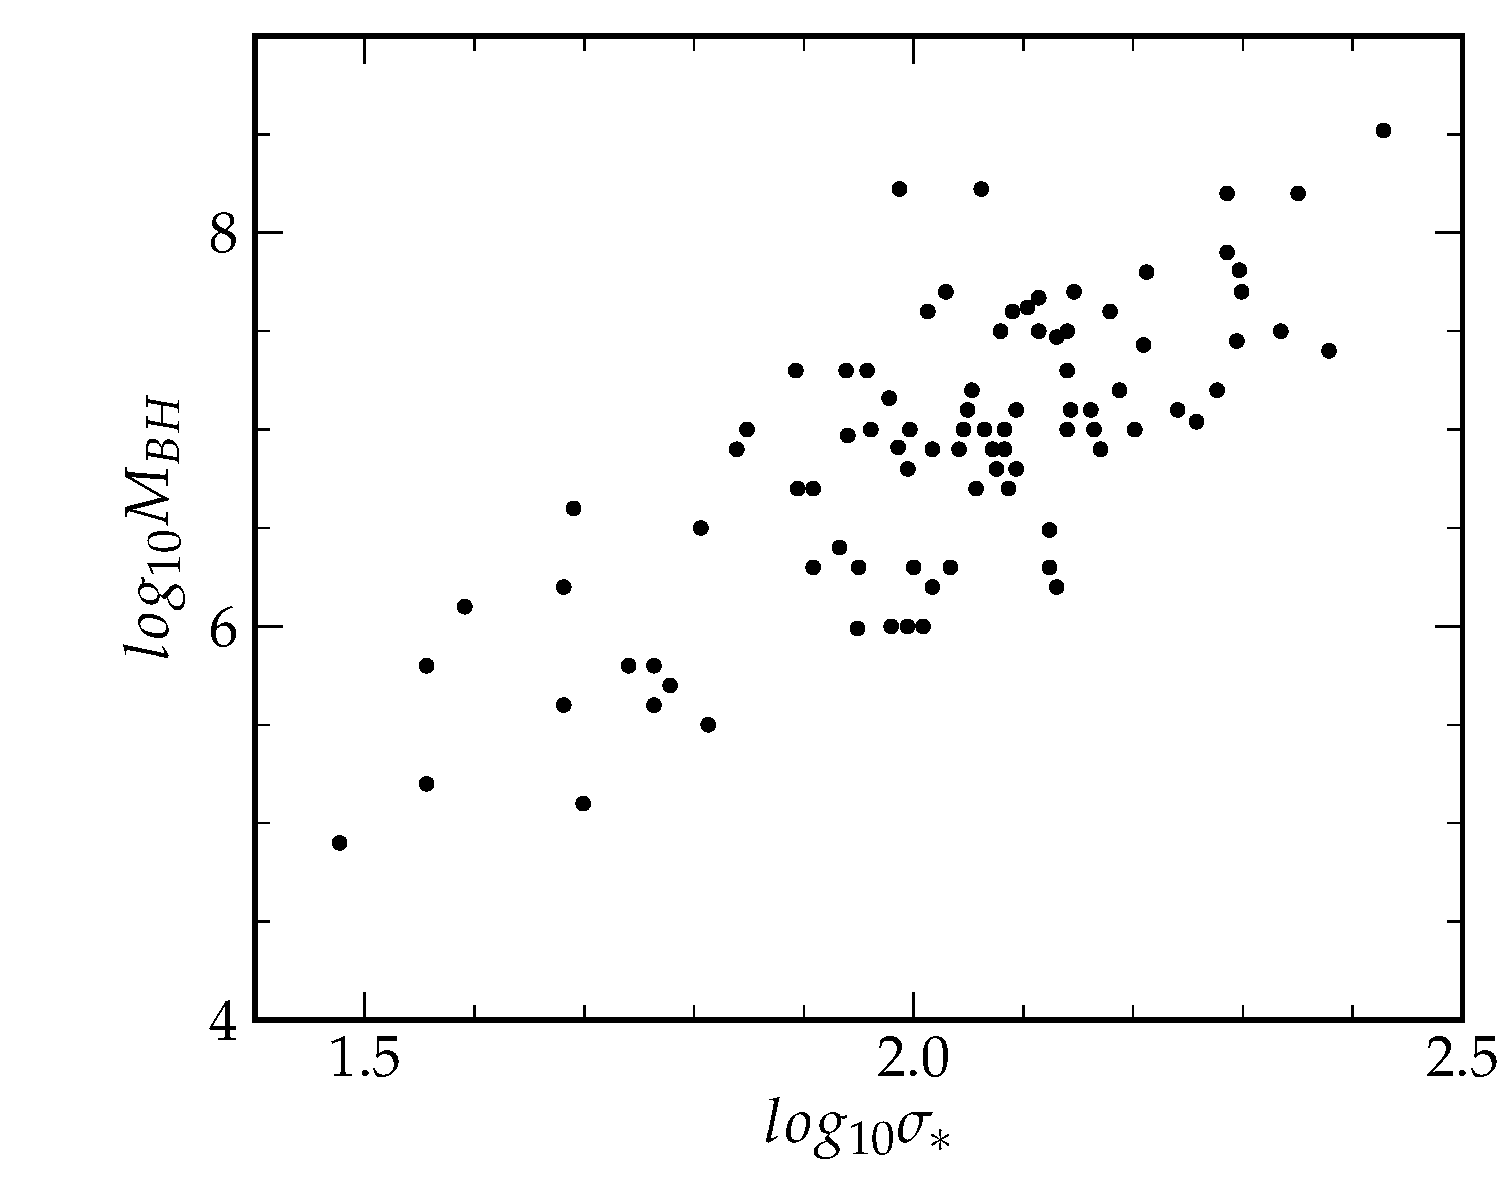
\includegraphics[width=0.5\textwidth]{1a.pdf}
\caption{Data loaded from the Ay190 website}
\label{fig:data}
\end{figure}

\subsection{Linear Regression - Ignoring Errors}

When doing a simple linear regression we simply take the least squares estimator
for the slope and for the intercept. We found in figure ~\ref{fig:linreg} 
that our line bisects the data nicely. It also appears that the errors are
evenly or even normally distributed which is again a good indicator of a good 
fit.

\begin{figure}[bth]
\centering
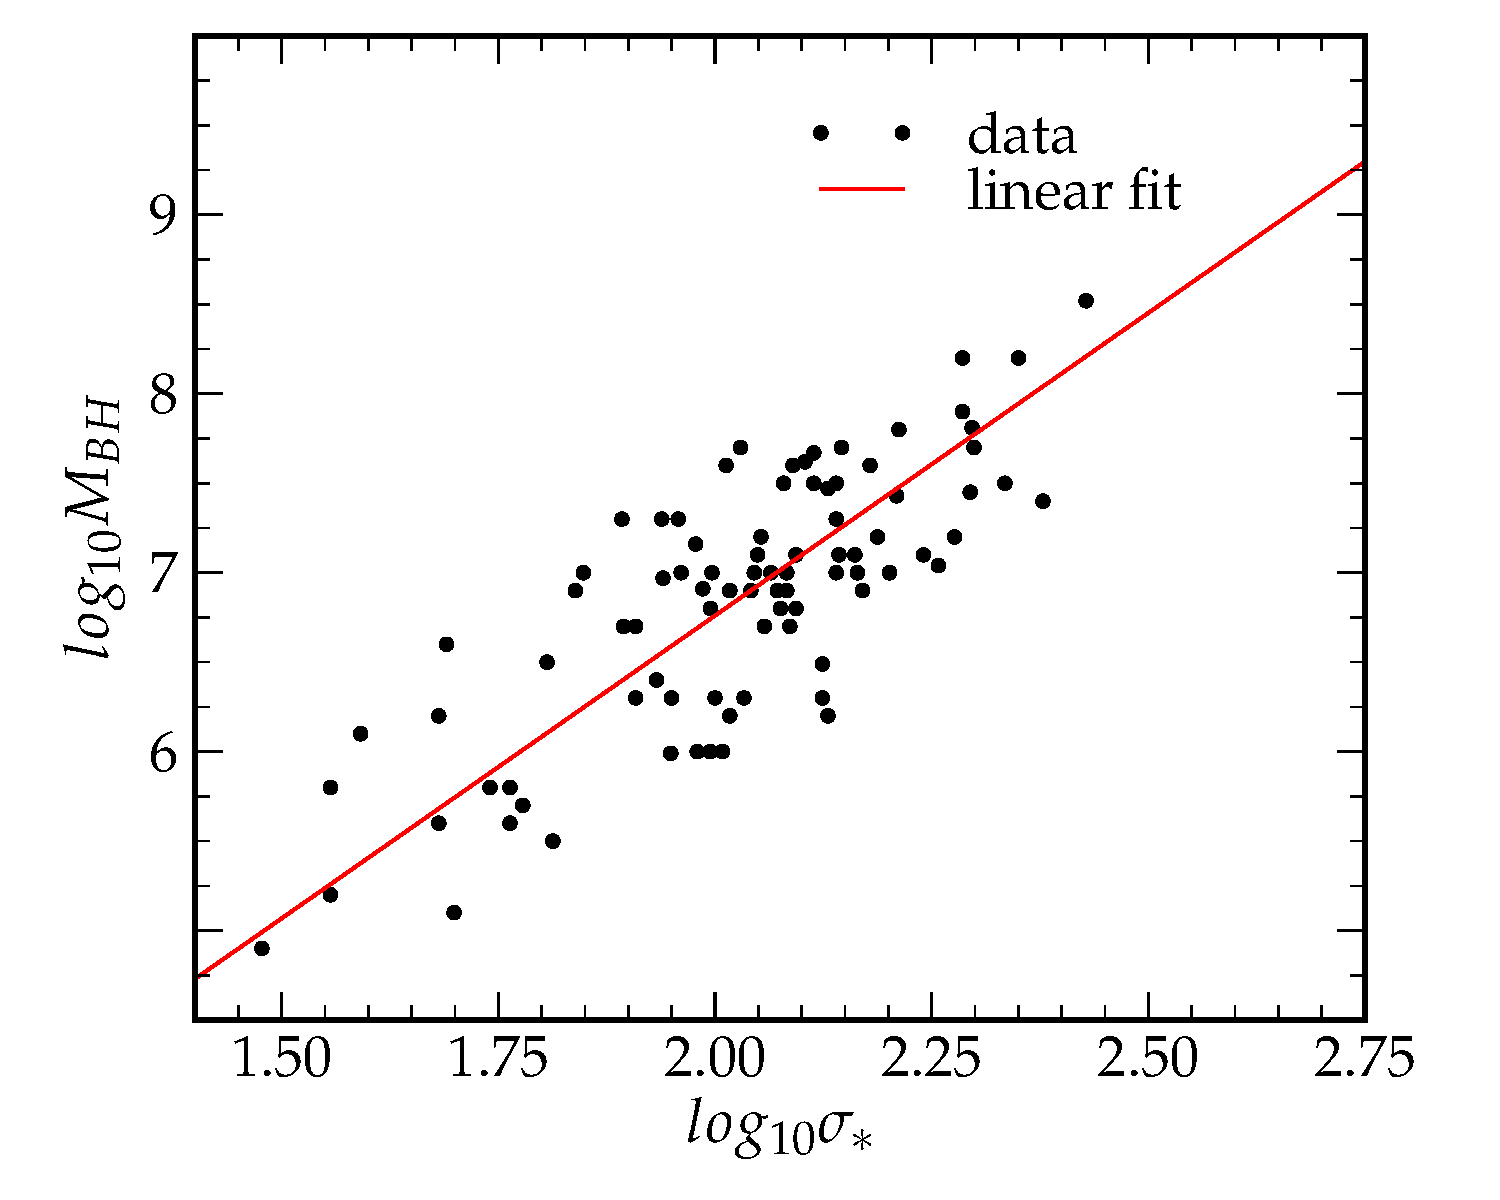
\includegraphics[width=0.5\textwidth]{1b.pdf}
\caption{We have succesfully implemented a linear fitter.}
\label{fig:linreg}
\end{figure}

\subsection{Linear Regreession - Including Errors}

When we add the error terms I chose to add the formal errors. We note that our
fit doesn't change too much but now the parameters of the fit have error. So
by taking the linear regression and $\pm \sigma$ in both intercept and slope 
gives us a sense of how confident we are in the initial fit. This gives us a 
more intuitive visual way of thinking about uncertanty in fits.

\begin{figure}[bth]
\centering
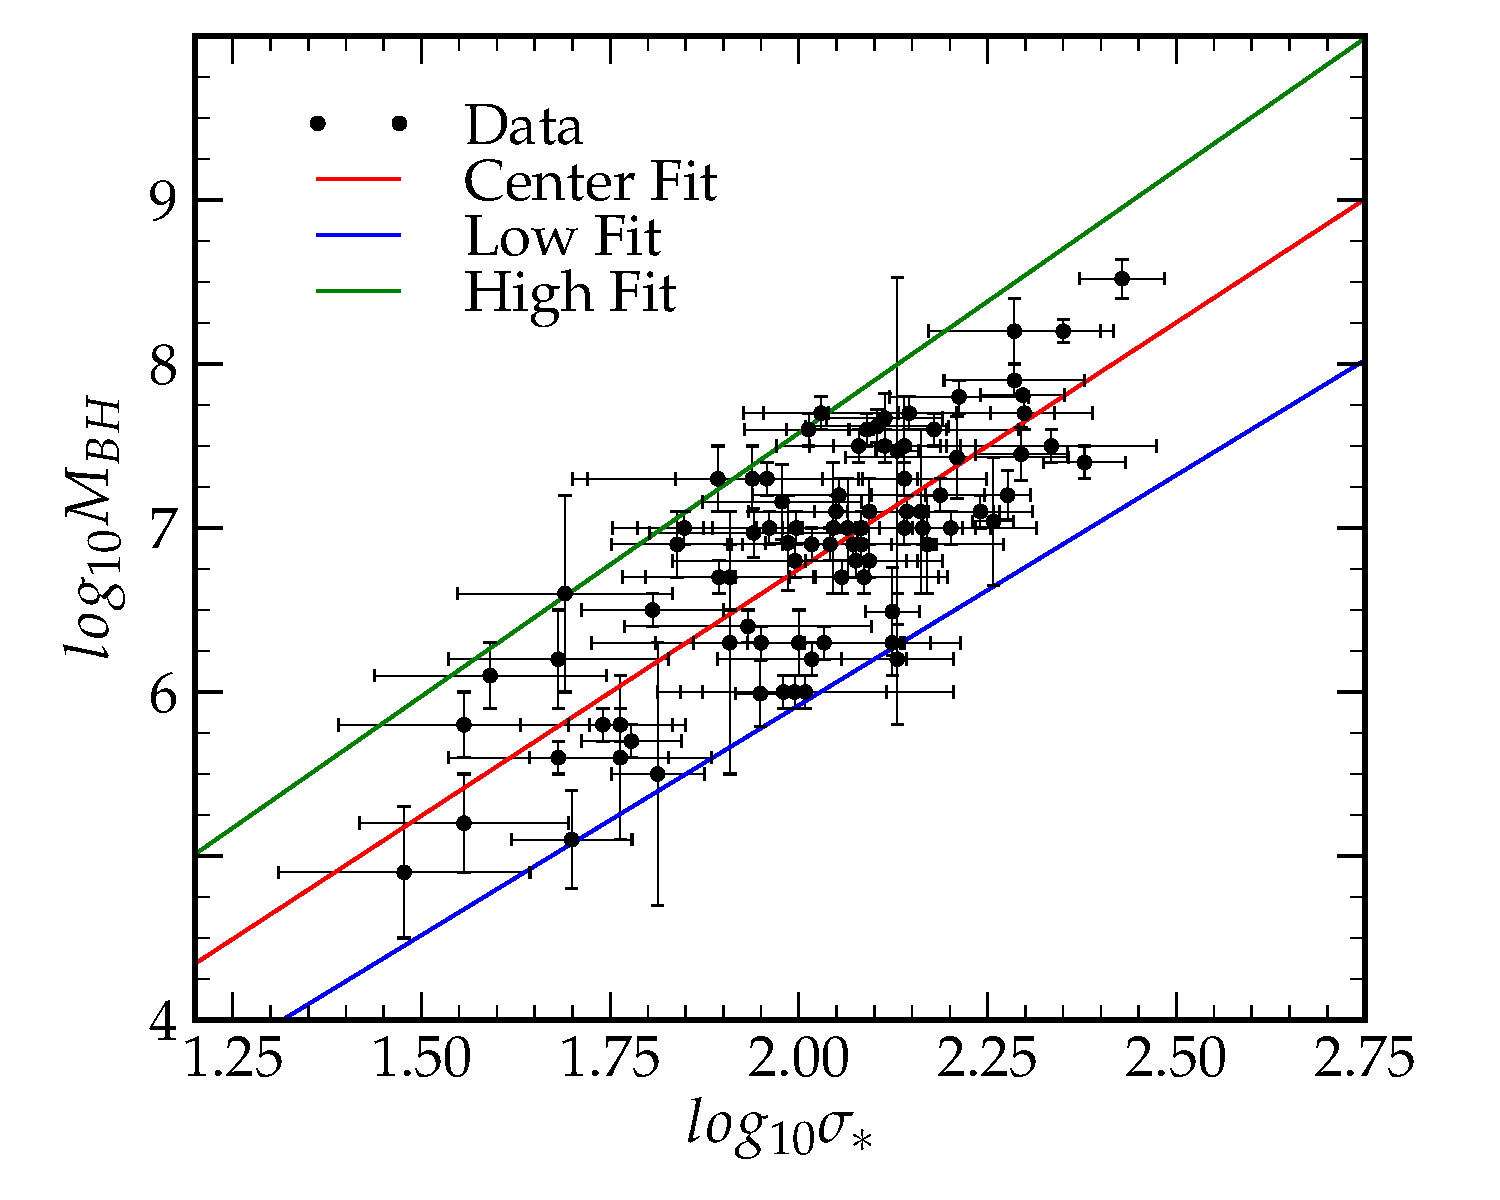
\includegraphics[width=0.5\textwidth]{1c.pdf}
\caption{Displays the $\pm \sigma_m \& \pm \sigma_b $ linear fits.}
\label{fig:dft}
\end{figure}


\end{document}




